\documentclass [a4paper, 12pt] {scrartcl}
\linespread{1.2}
\renewcommand{\familydefault}{\sfdefault}
\usepackage[framed,numbered,autolinebreaks,useliterate]{mcode}
\usepackage{amsfonts}
\usepackage{amsmath}
\usepackage{acronym}
\usepackage{amssymb}
\usepackage{longtable}
\usepackage{tabularx} 
\usepackage{graphicx, color} 
\usepackage{fancyhdr}
\usepackage[margin=1in,headsep=.6in]{geometry} 
\usepackage{rotating}	
\usepackage{wrapfig} 	
\usepackage{multirow}	
\usepackage{textcomp}
\usepackage[utf8]{inputenc} 
\usepackage{color}
\usepackage{caption} 
%\usepackage[ngerman]{babel}
\usepackage{booktabs}
\usepackage{epstopdf}
\usepackage[xindy,toc,nonumberlist,toc,section]{glossaries}
\usepackage{blindtext}
\usepackage{microtype}
\usepackage{color,siunitx}
\usepackage{todonotes}
\usepackage{subfig}
\usepackage{csquotes}
\usepackage{perpage}
\MakePerPage{footnote} 
\usepackage[backend=biber,natbib=true,hyperref=true,style=ieee]{biblatex} 
\addbibresource{PRObat.bib}
% Eigene definierte Zeichen
\newcommand{\sei}{\stackrel{!}{=}} % should be equal to
\newcommand{\cel}{$^{\circ}$C \ } % degrees celsius (text)
\newcommand{\mcel}{^{\circ}C \ } % degrees celsius (math)
\newcommand{\matlab}{Matlab\textsuperscript{\textregistered}} % Matlab with (R)
\newcommand{\java}{JAVA\textsuperscript{\texttrademark}} %  JAVA with TM
\newcommand{\subi}[1]{_\text{#1}} % subscript index
\newcommand{\subs}[2]{_{\text{#1}, #2}} % subscript index + running index
\newcommand{\dexp}[1]{\cdot 10^{#1}} % *10^...
% Multiline in table (left)
\newcommand{\tml}[1]{\begin{tabular}{@{}l@{}}#1\end{tabular}}
% Multiline in table (center)
\newcommand{\tmc}[1]{\begin{tabular}{@{}c@{}}#1\end{tabular}}
% Multiline in table (right)
\newcommand{\tmr}[1]{\begin{tabular}{@{}r@{}}#1\end{tabular}}
%Color definitions
\usepackage{xcolor}
\definecolor{HTWgreen}{RGB}{119,185,0}
\definecolor{grey}{RGB}{175,175,175}
\definecolor{TUred}{RGB}{197,14,31}
\definecolor{TUgrey}{RGB}{113,113,113}
\usepackage{sectsty}
\chapterfont{\color{TUred}}  % sets colour of chapters
\sectionfont{\color{TUred}}  % sets colour of sections
\subsectionfont{\color{TUgrey}}  % sets colour of sections
\usepackage[hidelinks, backref=true]{hyperref} 
\pagestyle{fancy}
\renewcommand{\sectionmark}[1]{\markright{\thesection.\ #1}}
%Heading
\lhead{\includegraphics[width=0.1\textwidth]{tulogo.pdf}}
%\rhead{\hspace{-0.14in}\vspace{-0.14in}\includegraphics[width=0.25\textwidth]{htwlogo}}
\chead{}
%Footer
\lfoot{}
\cfoot{\thepage} 
\rfoot{} 
\renewcommand{\headrulewidth}{0.4pt}
\renewcommand{\footrulewidth}{0.4pt} 
\captionsetup{format=hang,font=small,labelfont=bf,textfont=it,
	justification=justified,singlelinecheck=false}
\renewcommand{\thefootnote}{\roman{footnote}}
\begin{document}
\begin{titlepage}
	\begin{figure}
		\includegraphics[width=\textwidth]{GUI.png}
			\vskip 30px
		\begin{minipage}[b]{\textwidth}
			\flushright 
			{\LARGE\textbf{Cell Resolved \matlab\ OOP Model of a Lithium Iron Phosphate Battery Pack}}\\
			\vskip 10px
			\textbf{Marc Jakobi, Festus Anyangbe, Marc Schmitdt} \\
			\today \\
			HTW Berlin \\
			\vskip 10px
			Supervision: \\ \textbf{M.Sc. Steven Neupert}\\
			TU Berlin \\
			\vskip 10px
		\end{minipage}
	\end{figure}
\end{titlepage}
\clearpage
\begin{titlepage}
	\fancypagestyle{myheadings}{Inhalt}
	\tableofcontents
\end{titlepage}\clearpage
\setcounter{page}{1}
\pagenumbering{roman}
\listoffigures
\listoftables
\section*{Acronyms}
\thispagestyle{plain}
\markboth{Acronyms}{Acronyms}
\begin{acronym}
	\acro{BMS}[BMS] battery management system
	\acro{CCCV}[CCCV] constant current / constant voltage
	\acro{EOL}[EOL] end of life
	\acro{GUI}[GUI] graphical user interface
	\acro{JVM}[JVM] \java\ virtual machine
	\acro{MEX}[MEX] \matlab\ executable
	\acro{OO}[OO] object oriented
	\acro{OOP}[OOP] object oriented programming
	\acro{SP}[SP] strings of parallel elements
	\acro{std}[std] standard deviation
	\acro{PS}[PS] parallel strings
\end{acronym}
\section*{List of Symbols}
%\addcontentsline{toc}{chapter}{Formelverzeichnis} 	%Einbinden Des Verzeichnisses in das Inhaltsverzeichnis
\thispagestyle{plain}	%erste Seite des Kapitels ohne Kopfzeile
\markboth{List of symbols}{List of symbols}
\captionsetup{list=false}%captions werden nicht in die zugehörigen Verzeichnisse geschrieben

\begin{longtable}{lrl}
\captionlistentry{Symbol}\\
\toprule
Symbol		 					& Unit  	& Description \\
\midrule
$C\subi{dis}$					& Ah						& discharge capacity \\
$F$								& As/mol					& Faraday constant \\
$I$								& A							& Current \\
$SoC$							& \%						& state of charge \\
$R$								& J/(mol $\cdot$ K)			& universal gas constant  \\
$rmse$							& -							& root mean squared error \\
$T$								& K or \cel					& temperature \\
$V$								& V							& voltage \\
$z\subi{Li}$					& -							& ionic charge number of lithium \\
\bottomrule
\end{longtable}

\captionsetup{list=true}%captions werden in die zugehörigen Verzeichnisse geschrieben
\setcounter{table}{0}
\captionsetup{list=true}
\setcounter{table}{0}
\clearpage
\setcounter{page}{1}
\pagenumbering{arabic}


%% INCLUDES / SUBSECTIONS HERE
\markboth{Preface}{Preface}
\section*{Preface}
\addcontentsline{toc}{section}{Preface}
The following text provides a complete documentation of the battery model provided in the \mcode{lfpBattery} \matlab\ package. It combines a description of the model's components with an analysis and validation using example simulations and a tutorial on how to use the package.

\subsection*{Organization}
\addcontentsline{toc}{subsection}{Organization}
This documentation is organized in sections that are sorted in such a way that a detailed understanding of the model's design and functionality is conveyed to the reader. For a basic knowledge of how to use the model, the sections do not have to be read in order. Parts of the documentation that are not relevant to the usage of the model in \matlab\ can safely be skipped. However, it is recommended to read the entire documentation for an understanding of the strengths and weaknesses of the model.

\subsection*{Typing conventions of this documentation}
\addcontentsline{toc}{subsection}{Typing conventions of this documentation}
Since this documentation describes a \matlab\ package, the following special text formatting is used extensively:
\begin{itemize}
	\item \matlab\ code and the names of \matlab\ objects and properties are formatted in \mcode{fixed-width} font and the default \matlab\ colour coding.
	\item \matlab functions (methods) are formatted in \mcode{fixed-width} font with brackets added at the end, e.g. \mcode{plot()}.
	\item Formulas, mathematical symbols, physical units and constants are formatted according to the norms DIN~1338, DIN~1304, DIN~1301 and DIN~1313.
	\item If a formula, symbol, unit or constant is used within \matlab\ code, the \mcode{fixed-width} font is used.
\end{itemize}

\subsection*{Quick start}
\addcontentsline{toc}{subsection}{Quick start}
To quickly get started with the usage of this package, skip to the sections~\ref{sec:batteryPack} and~\ref{sec:GUI}. Note that any script or function that uses this package should start with the line
\begin{lstlisting}
import lfpBattery.*
\end{lstlisting}
Alternatively, only the required objects can be imported, e.g.
\begin{lstlisting}
import lfpBattery.batteryPack lfpBattery.dischargeCurves
bat = batteryPack(varargin{:});
dC = dischargeCurves(varargin{:});
\end{lstlisting}
or the object with the name \mcode{objectName} can be initialized as \mcode{lfpBattery.objectName}, e.g.
\begin{lstlisting}
bat = lfpBattery.batteryPack(varargin{:}); % creates a batteryPack object
\end{lstlisting}
For the code examples provided in this documentation, it is assumed that the \mcode{lfpBattery} package has been imported. \\
Section~\ref{sec:GUI} provides a description of the GUI tools that can be used for getting to know the package and for creating the required curve fits. For repeaded use in a simulation, it is recommended to start off with the \mcode{batteryPack} class, which provides centralized access to almost all of the features of this package and is described in section~\ref{sec:batteryPack}.

\subsection*{Terminology}
\addcontentsline{toc}{subsection}{Terminology}
Object oriented programming (OOP), design pattern and \matlab\ terminology is used frequently throughout this documentation. A short description of some of the terms is provided in the following.

\subsubsection*{Interface} \label{sec:interface}
In OOP languages such as \java and C++, the term "interface" commonly refers to an abstract set of methods that specifies the behaviour that objects must implement. Unlike a class, an interface does not have any properties. \matlab\ OOP contains abstract classes, but no interfaces. However, in the terminology of design patterns, an interface can also be an abstract class. In this documentation, an abstract class that defines the behaviour that objects must implement via a set of methods and/or properties is referred to as an "interface". Examples are the \mcode{curveFitInterface} for all curve fitting classes and the \mcode{batteryInterface}, which is a common interface for the battery pack elements and the cells.

\subsubsection*{Immutable}
In \matlab\ OOP, object properties can be private (read only) or public (read and write access), among others. A property that can be set from an object's constructor (upon initialization), but is read only afterwards is called "immutable".

\subsubsection*{Observer}
In the Observer design pattern, an observer is an object that is notified by the subject it is observing when an event occurs. The subject sends information to the observer about which event has occurred, the source of the event and which of the observer object's methods is to be triggered. Observers are also often referred to as "listeners".

\subsubsection*{Subject}
In the Observer design pattern, a subject is an object that is observed. It holds a handle reference to one or more observers and when an event occurs, it sends out a notification to the observer, triggering one or more of it's methods.

\subsubsection*{Component}
In the Composite design pattern, a component is any class that implements the shared interface. Both composite and leaf elements are components.

\subsubsection*{Composite}
In the Composite design pattern, a composite is a component that can hold a reference to another component.

\subsubsection*{Leaf}
In the Composite design pattern, a leaf is a component that cannot hold a reference to another component.
\markboth{Introduction}{Introduction}
\section{Introduction}
In recent years, energy storage has been playing a more and more important role in various sectors. With the rapid advances in lithium-ion technology, the costs of lithium-ion batteries have been decreasing and their usage increasing steadily. Today, they are applied in many fields, e.g. Electric vehicles, storage in combination with photovoltaic systems, grid stabilization, etc. The various applications result in different operation strategies and stress factors, which often need to be modelled. The modelling of batteries makes it possible to simulate the behaviour of existing technologies while designing a system (i.e. with the purpose of determining the ideal type and size of the battery). It also plays an important role in the further development of the technologies themselves (i.e. of battery management systems). \\
Most battery models can be classified into 3 categories: (i) Theoretical, (ii) semi-empirical and (iii) empirical models~\cite{cui_multi-stress_2015, xu_degradation-limiting_2013}. The most precise approach is theoretical modelling, in which it is attempted to simulate the physical processes within the battery. Such processes could be the transfer of lithium ions through the electrolyte or the ageing mechanisms, e.g. lithium plating. A negative aspect of theoretical modelling is the complexity, which results in a high resource demand and thus slow simulations. A positive aspect is the fact that theoretical models can be adapted to any type of battery. The resource demand is significantly reduced with empirical models, in which certain behaviour is represented by equivalent circuits that are parametrised from measurements. However, simplifications must be made to a certain degree and an empirical model of one battery cannot be easily transferred to another, because the measurements have to be recorded for every model. In the worst-case scenario, the measured data might differ so strongly that the model has to be changed completely. The model used in this package takes a semi-empirical approach, in which the pros of the theoretical and empirical approaches are combined. The only con is the necessity of simplifications. Theoretical phenomena are used to model measured data, which allows for easy adaptation of the model to different technologies with low resource consumption. \\
A motivation for this project is the scarcity of detailed, cell-resolved simulation models and the almost complete lack of open-source models. Furthermore, most \matlab\ simulations appear to be designed in a procedural style. Object oriented (OOP) programming in \matlab\ still seems to be a rare phenomenon today, although advanced OOP capabilities were introduced as early as version R2008a~\cite{foti_inside_2008}. This may in part be due to the fact that Matlab classes are often thought of as slow (with long method overhead times). However, the just-in-time compiler\footnote{Matlab's code execution mechanism.} (JIT) was overhauled in \matlab\ R2016a, resulting in an OOP performance increase of up to 40~\% compared to the predecessor~\cite{_matlab_2016}. It can be assumed that OOP performance will only increase further with newer releases. The approach chosen for this open-source model combines the flexibility of OOP design patterns with Matlab's highly optimized double-precision general matrix-matrix multiplication (dgemm) libraries.
\markboth{Discharge curves}{Discharge curves}
\section{Discharge curves} \label{sec:dischargeCurves}
Many battery data sheets provide measured discharge curves, on which the charging and discharging behaviour of this model is based. Rather than determining the curves according to the internal impedance, a common approach \cite{lijun_gao_dynamic_2002}, this model determins the curves directly by means of digitizing the images and creating a curve fit. The classes used for fitting and modelling the discharge curves are described in the following subsections.

\subsection{Single discharge curve}
For modelling a single discharge curve, the class \mcode{dischargeFit} is used, which implements the interface \mcode{curveFitInterface}\todo{Section describing interface, etc.}. The curve is fitted according to \cite{werder_entwicklung_2014}, using a function that is loosely based on the Nernst equation with two exonential functions superimposed as a correction for the voltage drops at the beginning and end of the curve.
\begin{equation}
\begin{aligned}
V(SoC) = x_1 - \frac{R\cdot T}{z\subi{Li}\cdot F}\cdot ln\Big(\frac{SoC}{1-SoC}\Big)
+ x_2\cdot SoC + x_3 \\
+ (x_4 + (x_5 + x_4\cdot x_6)\cdot SoC)\cdot exp(-x_6\cdot SoC) \\
+ x_7\cdot exp(-x_8\cdot SoC)
\end{aligned}
\end{equation}

where $x_1,\ ..,\ x_8$ are the fit parameters, $R = 8.3144598$ J/(mol $\cdot$ K) is the universal gas constant, $z\subi{Li} = 1$ is the ionic charge number of lithium, $F = 96485.3328959$ As/mol is the Faraday constant, $SoC$ is the state of charge, $V$ is the voltage in V and $T$ is the temperature in K at which the curve was recorded. The curves are fitted using the levenberg-marquardt algorithm and either the \mcode{lsqcurvefit} method, the \mcode{fminsearch} method or a combination of both, depending on the user's preference. 

\subsubsection{Object creation}
A \mcode{dischargeFit} object is created with the digitized raw data - the voltage $V$ in V, the discharge capacity $C\subi{dis}$ in Ah, the current $I$ in A at which the curve was recorded and the temperature $T$ in K at which the curve was recorded.
\begin{lstlisting}
d = dischargeFit(V, C_dis, I, T);
\end{lstlisting}
\mcode{V} and \mcode{C_dis} are vectors containing the digitized raw data from the data sheet. Further options, such as initial values for the fit parameters $x_1,\ ..,\ x_8$ and the fit method can be passed to the constructor using Matlab's name-value pair syntax:
\begin{lstlisting}
d = dischargeFit(V, C_dis, I, T, 'OptionName', OptionValue);
\end{lstlisting}
By default, the initial fit parameters are set to zero and the curve is fit by first using \mcode{lsqcurvefit}, followed by \mcode{fminsearch}. The initial fit parameters are stored in a vector \mcode{x0} of \mcode{length} 8, which can be passed via the option name \mcode{'x0'}, for example using the following syntax:
\begin{lstlisting}
x0 = ones(8, 1);
d = dischargeFit(V, C_dis, I, T, 'x0', x0);
\end{lstlisting}
The method used for the curve fitting can be passed to the constructor using the option name \mcode{'mode'}. The corresponding value must be one of the following three strings:
\begin{itemize}
	\item \mcode{'lsq'} for \mcode{lsqcurvefit}
	\item \mcode{'fmin'} for \mcode{fminsearch}
	\item \mcode{'both'} for \mcode{lsqcurvefit} followed by another fit using \mcode{fminsearch}
\end{itemize}
e.g.
\begin{lstlisting}
d = dischargeFit(V, C_dis, I, T, 'mode', 'fmin');
d.plotResults
\end{lstlisting}
Depending on the curve and on the technology, one of the methods may return a better result.

\subsubsection{Visual validation}
A visual validation can be performed by calling the class's \mcode{plotResults} method (see above). In Figure~\ref{fig:dischargeFit01}, the results of two \mcode{dischargeFit} objects using the same raw data are compared.
\begin{figure}[b!]
	\captionsetup{type=figure}
	\centering
	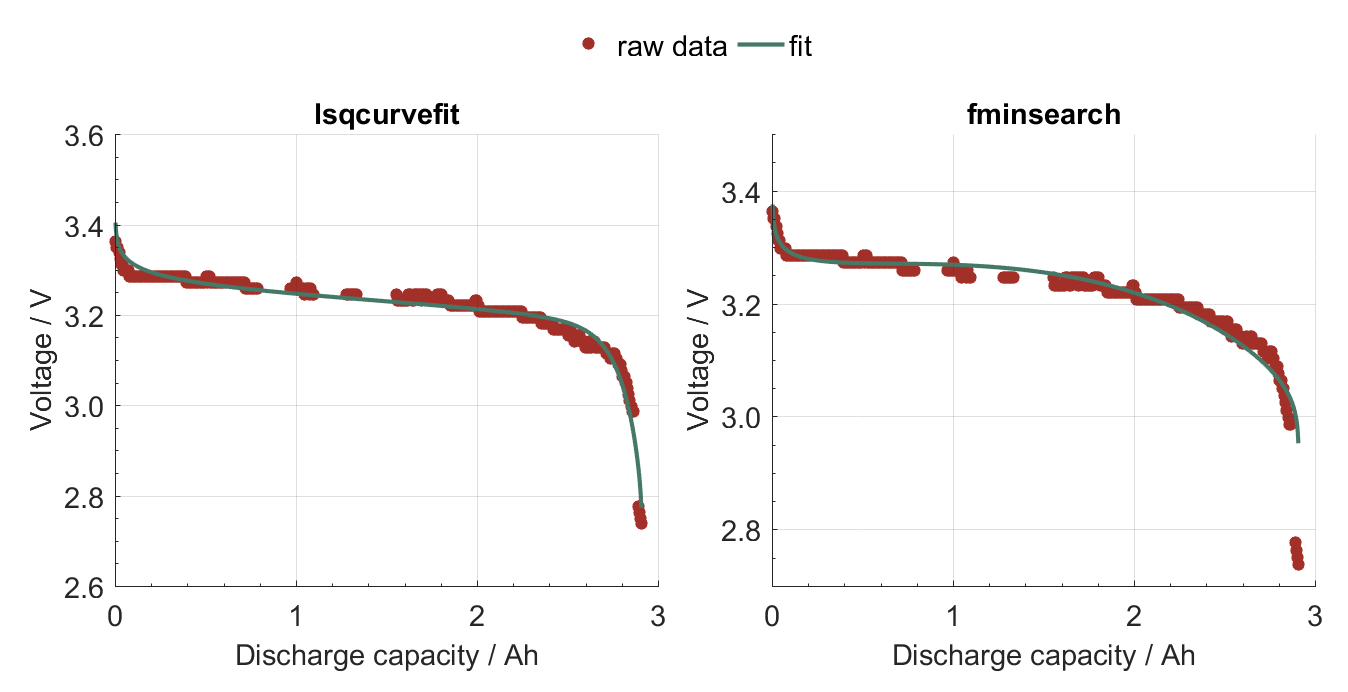
\includegraphics[width=.97\textwidth]{dischargeFit01}
	\caption[Fit results of the \mcode{dischargeFit} class using the fit methods \mcode{lsqcurvefit} and \mcode{fminsearch}, respectively]{Fit results of the \mcode{dischargeFit} class using the fit methods \mcode{lsqcurvefit} and \mcode{fminsearch}, respectively. The raw data was extracted from \cite{_data_2010}.}
	\label{fig:dischargeFit01}
\end{figure}
\begin{figure}[t!]
	\captionsetup{type=figure}
	\centering
	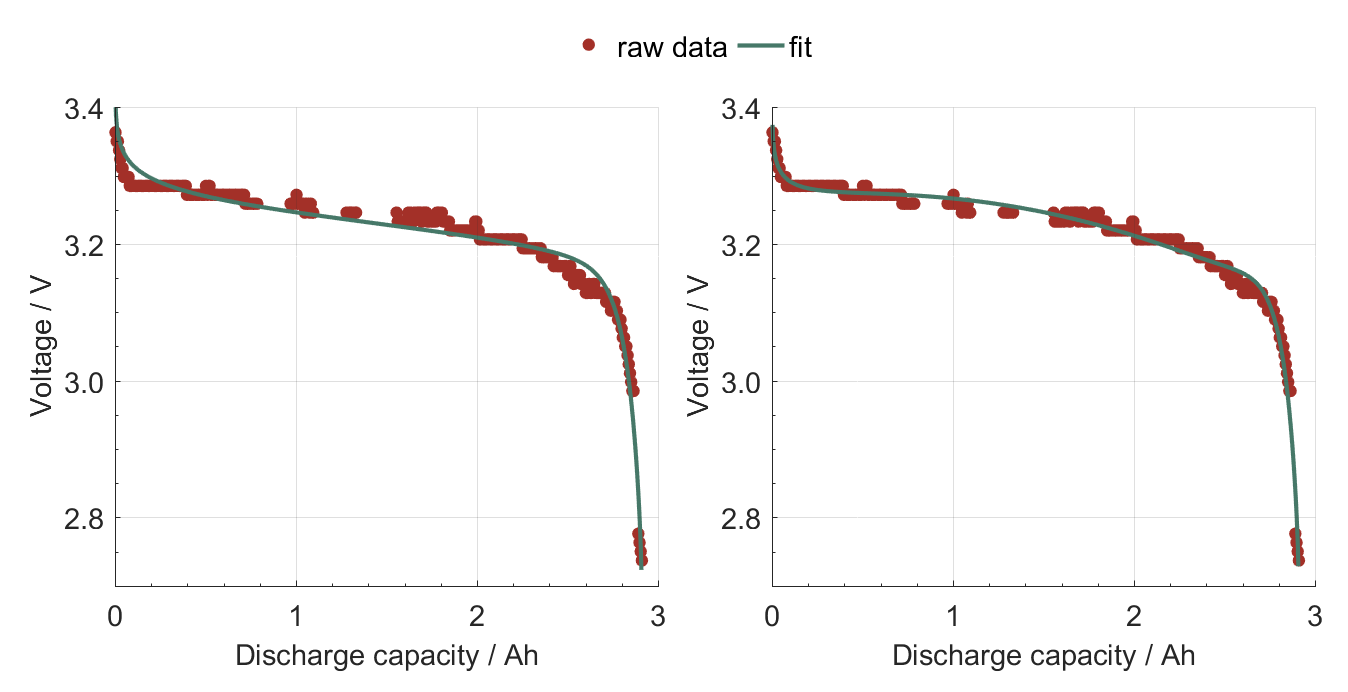
\includegraphics[width=.97\textwidth]{dischargeFit02}
	\caption[Fit results of the \mcode{dischargeFit} class using the fit mode \mcode{'both'} with the default parameter initialization and with a custom parameter initialization]{Fit results of the \mcode{dischargeFit} class using the fit mode \mcode{'both'} with the default parameter initialization (left) and with a custom parameter initialization (right). The raw data was extracted from \cite{_data_2010}.}
	\label{fig:dischargeFit02}
\end{figure}

In this example, \mcode{'lsq'} appears to return better results for the voltage drop at the end of the curve, while \mcode{'fmin'} results in a more precise fit for the voltage drop at the beginning of the curve. Further differences can be seen in the fits' curvatures. 
The \mcode{'lsq'} option results in a slightly flatter curve than the \mcode{'fmin'} mode. The results of a \mcode{dischargeFit} object using the \mcode{'both'} option are presented in Figure~\ref{fig:dischargeFit02}.
Using the default fit parameter initialization of \mcode{zeros} (left) appears to improve the curvature and voltage drops slightly, compared to the other modes. Further improvements can be made by passing custom initial fit parameters to the constructor via the option \mcode{'x0'} (see Figure~\ref{fig:dischargeFit02}, right).

\subsubsection{Object properties}
Further fit quality analysis can be performed via the root mean squared error $rmse$, the mean difference in voltage between the raw data and the curve fit at the respective positions of the raw data $\overline{\Delta V}$ in V and the maximum difference between the raw data and the curve fit at the respective positions $\Delta V\subi{max}$ in V.
The $rmse$ for a curve fit with the raw data $y\subi{raw}$ and the fitted data $y\subi{fit}$ at the same $x$ coordinates is defined as
\begin{equation}
rmse = \sqrt{\sum_{i = 1}^{n}(|y\subs{raw}{i}-y\subs{fit}{i}|)^2}
\end{equation}
where $i$ is the index of the measurement and $n$ is the number of measurements.
\markboth{Age model}{Age model}
\section{Age model}
The age model is implemented using the Observer design pattern. This way, various age models (predefined or custom) can be dynamically added to a battery model at run time or even left out completely. The event oriented age model provided in this package is based solely on cycle counting, for which A mathematical approach developed by~\cite{dambrowski_mathematical_2012} is implemented. A description of the counting algorithm and the classes used to implement the age model is provided in the following sections.
\subsection{Cycle counter}
Cycle counting algorithms are designed to count cycles from a set of measured data. A challenge for a running simulation or a battery management system (BMS) that relies on cycle counting is to decide when to count the cycles of an accumulated data set. Counting could be done at fixed time intervals or it could be triggered by a certain event. The latter is the approach implemented by the \mcode{cycleCounter} interface.
\subsubsection{The \mcode{cycleCounter} interface}
The observing of charge cycles is handled by the abstract \mcode{cycleCounter} interface, in which all methods except for the \mcode{count()} method are predefined.
\markboth{Battery Composition}{Battery Composition}
\section{Battery Composition}
The battery pack is modelled using a variation of the Composite design pattern with multiple composite classes\footnote{The basic Composite design pattern has one component interface, one composite class and one leaf class.}. This way, cells can be combined flexibly in various different topologies.

\subsection{Overview}
\label{sec:batteryCompositionOverview}
The \mcode{batteryInterface} is the abstract component that defines the interface for all objects in the composition. It is subclassed by all other battery elements. The \mcode{batteryCell} objects are the "leaves" and a composite can be one of the following classes:
\begin{itemize}
	\item \mcode{parallelElement}: A set of components in parallel.
	\item \mcode{seriesElementAE}: A set of components in series with active equalization.
	\item \mcode{seriesElementPE}: A set of components in series with passive equalization.
\end{itemize}
Each component can either be another composite object or a leaf.
\begin{figure}[b!]
	\captionsetup{type=figure}
	\centering
	\includegraphics[width=\textwidth]{topologies2.pdf}
	\caption[Visualization of the possible battery topology compositions]{Visualization of the possible battery topology compositions.}
	\label{fig:topologies2}
\end{figure}
Figure~\ref{fig:topologies2} provides a visual overview of the topologies that are possible using different compositions. Using this variation of the Composite design pattern, the components can be combined in any possible way at runtime. The most common battery topologies are strings of parallel elements (SP) and parallel strings of cells (PS)~\cite{cordoba-arenas_control-oriented_2015}. In Figure~\ref{fig:topologies2}, these would be the case if the composition's leaf nodes (cells) were all in the second layer (marked green). However, since every component can be either a cell or another composite, more complicated topologies are made possible in this package. \\
\begin{figure}[t!]
	\captionsetup{type=figure}
	\centering
	\includegraphics[width=\textwidth]{composite_schema.pdf}
	\caption[Class diagram of the battery composition with communication flows and inheritance links]{Class diagram of the battery composition with communication flows and inheritance links.}
	\label{fig:composite_schema}
\end{figure}

\subsection{Method delegation}
A pattern diagram of the classes used for the topology composition is depicted in Figure~\ref{fig:composite_schema}. Every composite element holds a reference to a component and delegates the methods called on it to said component. The delegated methods are wrapped with the rules of the respective topology in a similar fashion as is done with the Decorator design pattern. An example of the method delegation for a PS configuration - a \mcode{parallelElement} that holds a set of \mcode{seriesElement} objects, each in turn holding a set of \mcode{batteryCell} objects - is visualized in Figure~\ref{fig:method_delegation}. In this example, a current \mcode{I} and the simulation time step size is passed to the \mcode{parallelElement} via a \mcode{getVoltage()} method. The \mcode{parallelElement} determines which portion of \mcode{I} to send to each of it's components and delegates the method. Each \mcode{seriesElement} does the same and delegates the method to it's \mcode{batteryCell} objects. These return their voltages back to the \mcode{seriesElement} objects, which sum up the results received from their cells and pass the sum back to the \mcode{parallelElement}. Finally, the \mcode{parallelElement} calculates the mean of all the summed up voltages it received and passes the end-result back to the client.
\begin{figure}[t!]
	\captionsetup{type=figure}
	\centering
	\includegraphics[width=\textwidth]{method_delegation.pdf}
	\caption[Example of a method being delegated across a battery pack composition]{Example of a method being delegated across a battery pack composition.}
	\label{fig:method_delegation}
\end{figure}
The following operations are delegated by an object that implements the \mcode{batteryInterface}:
\begin{itemize}
	\item Determination of the new voltage after charging or discharging a with a certain current and time step size. This is delegated to each \mcode{batteryCell} object's \mcode{dischargeCurves} reference.
	\item Charging or discharging the battery.
	\item Determining the state of the battery if it were to be charged or discharged.
	\item Determining the maximum charging or discharging current.
	\item Calculating the pack's $SoH$.
	\item Getters and setters for the component's voltage and capacity properties.
	\item Getter for the component's internal impedance. 
\end{itemize}
With the number of subcomponents $n$, a component's voltage is determined as
\begin{equation} 
V\subi{component} = \left\lbrace
\begin{smallmatrix}
\frac{\sum_{i=1}^{n}V\subs{subcomponent}{i}}{n} & \text{for a parallel element}\\
& \\
\sum_{i=1}^{n}V\subs{subcomponent}{i} & \text{for a series element} \\
\end{smallmatrix}
\right.
\end{equation}
And a component's capacity is
\begin{equation}
C\subi{component} = \left\lbrace
\begin{smallmatrix}
\sum_{i=1}^{n}C\subs{subcomponent}{i} & \text{for a parallel element}\\
& \\
\min_{i=1}^{n}C\subs{subcomponent}{i} & \text{for a series element with passive equalization} \\
& \\
\frac{\sum_{i=1}^{n}C\subs{subcomponent}{i}}{n} & \text{for a series element with active equalization}\\
\end{smallmatrix}
\right.
\end{equation}
Since the $SoH$ is derived directly from the capacity (see Equation~\ref{eq:age_soh}), a component's $SoH$ can be determined in the same fashion.
\begin{equation}
SoH\subi{component} = \left\lbrace
\begin{smallmatrix}
\sum_{i=1}^{n}SoH\subs{subcomponent}{i} & \text{for a parallel element}\\
& \\
\min_{i=1}^{n}SoH\subs{subcomponent}{i} & \text{for a series element with passive equalization} \\
& \\
\frac{\sum_{i=1}^{n}SoH\subs{subcomponent}{i}}{n} & \text{for a series element with active equalization}\\
\end{smallmatrix}
\right.
\end{equation}
Due to the fact that the model is based on curve fits, the internal impedance $Z\subi{i}$ property is not used for modelling the charging behaviour directly. It does however, determine how the voltages and currents are distributed across the subcomponents when charging or discharging. The impedance proportionality factor $p\subi{z}$ of a subcomponent with index $j$ is the component's $Z\subi{i}$ divided by the sum of all subcomponents' $Z\subi{i}$.
\begin{equation}
p\subs{z}{j} = \frac{Z\subs{i}{j}}{\sum_{i=1}^{n}Z\subs{i}{i}}
\end{equation}
When charging, a series element with active equalization will distribute it's voltage equally across all of it's subcomponents to account for balancing, while a series element with passive equalization will distribute it's voltage according to $p\subs{z}{j}$. For a parallel element, the current is distributed in such a way that the subcomponent $j$ with the lowest $Z\subi{i}$ receives the highest current.
\begin{equation}
I\subs{subcomponent}{j} = \frac{\frac{1}{p\subs{z}{j}}}{\sum_{i=1}^{n}\frac{1}{p\subs{z}{i}}}
\cdot I\subi{component}
\end{equation}


\subsection{Battery Interface}
The battery interface is described in the following subsections. Every component implements the \mcode{batteryInterface}, so the methods described in this section can be called on \mcode{batteryCell} objects and on the composites.

\subsubsection{Battery object initialization}
To initialize a battery object at runtime, the nominal capacity $C\subi{n}$ in Ah and the nominal voltage $V\subi{n}$ in V must be passed to a \mcode{batteryCell} constructor. A composite can be initialized as an "empty" circuit element and the cell (or other composites) can be added to it via it's \mcode{addElements()} method\footnote{Here, "empty" is referred to in the sense of not holding any cells, not in the sense of an empty \matlab\ variable.}.

\begin{lstlisting}
% Initialize an "empty" parallel element
bat = parallelElement;
Cn = 3; % Nominal cell capacity in Ah
Vn = 3.2; % Nominal cell voltage in V
% Initialize 3 battery cells and add them to bat
for i = 1:3
	b = batteryCell(Cn, Vn);
	bat.addElements(b);
end
\end{lstlisting}
The \mcode{addElements()} method also accepts component arrays...
\begin{lstlisting}
for i = 1:3
	b(i) = batteryCell(Cn, Vn);
end
bat.addElements(b);
\end{lstlisting}
...and multiple inputs:
\begin{lstlisting}
b1 = batteryCell(Cn, Vn);
b2 = batteryCell(Cn, Vn);
b3 = batteryCell(Cn, Vn);
bat.addElements(b1, b2, b3);
\end{lstlisting}
To create a composition like the example in Figure~\ref{fig:method_delegation} (see also Figure~\ref{fig:topologies2}, right), the following syntax could be used:
\begin{lstlisting}
% Initialize "empty" parallel element
bat = parallelElement;
% Initialize 3 "empty" series elements each holding 3 cells
for i = 1:3
	se = seriesElementPE; % passive equalization
	for j = 1:3
		se.addElements(batteryCell(Cn, Vn))
	end
	% Add series elements to bat
	bat.addElements(se)
end
% Further initialization operations, e.g. bat.addcurves() here...
\end{lstlisting}

\subsubsection{Battery charging and discharging}
Battery charging \footnote{Discharging will also be referred to as charging (with a negative current) in this documentation.} is handled by the methods \mcode{powerRequest()} and \mcode{currentRequest()}. Both functions are called in a similar manner. The syntax is as follows:
\begin{lstlisting}
[P, V, I] = bat.powerRequest(P, dt);
[P, V, I] = powerRequest(bat, P, dt); % equivalent
[P, V, I] = bat.currentRequest(I, dt);
[P, V, I] = currentRequest(b, I, dt); % equivalent
\end{lstlisting}
Where \mcode{P} is the requested power $P$ in W, \mcode{I} is the requested current $I$ in A and \mcode{dt} is the simulation time step size $\Delta t\subi{s}$ in s. The methods return the actual power throughput in W, the battery's voltage $V$ at the end of the time step and the actual current throughput in A. The returned power and current is limited by the $SoC$ or the cells' maximum currents, among other factors.
\begin{figure}[b!]
	\captionsetup{type=figure}
	\centering
	\includegraphics[width=\textwidth]{powerRequest.pdf}
	\caption[Flow chart of the \mcode{powerRequest()} and \mcode{currentRequest()} methods]{Flow chart of the \mcode{powerRequest()} and \mcode{currentRequest()} methods.}
	\label{fig:powerRequest}
\end{figure}
Figure~\ref{fig:powerRequest} contains a flow chart of the charging process. The client sends a request to the battery. If the requested power is not equal to zero and the battery's $SoC$ is not already at it's upper or lower limit, a charge iteration is performed (the \mcode{iteratePower()} and \mcode{iterateCurrent()} methods are called, respectively) and the resulting power, current and voltage are returned to the client. A positive input to the charge iteration  indicates charging and a negative input specifies discharging. If the request is zero, signalling that the battery is in an idle state, a logical flag is set to true and the charge iteration is called with the battery's self-discharge $P\subi{sd}$. The logical flag is checked after every call to the charge iteration methods in order to return a power and current of zero to the client if it was set to true. If the $SoC$ is either at it's upper or lower limit, the battery simply returns it's voltage along with a power and current of zero.\\
\begin{figure}[t!]
	\captionsetup{type=figure}
	\centering
	\includegraphics[width=\textwidth]{iteratePower.pdf}
	\caption[Flow chart of the \mcode{iteratePower()} method]{Flow chart of the \mcode{iteratePower()} method.}
	\label{fig:iteratePower}
\end{figure}
A flow chart of the \mcode{iteratePower()} method is depicted in Figure~\ref{fig:iteratePower}. First, a current is estimated from the requested power and the battery's voltage. The current and the time step size are then delegated to the battery cells' \mcode{dischargeCurves} objects, in order to determine the resulting voltage. An approximation of the power is determined from the mean of the returned voltage and the battery's old voltage. This is repeated through recursion until the difference between the iterated power and the originally requested power meets a certain tolerance. If the resulting current is greater than the battery's maximum current $I\subi{max}$, the \mcode{iterateCurrent()} method is called using $I\subi{max}$ as an input. It's output current, the resulting power and voltage are returned. Otherwise, the $SoC$ is determined and compared the battery's upper and lower limit. If the $SoC$ is within the interval $[SoC\subi{min}, SoC\subi{max}]$, the power, current and voltage are returned. Otherwise, the requested power is adjusted according to the difference between the $SoC$ and the respective limit that was exceeded, thus starting the iteration again. \\
\begin{figure}[t!]
	\captionsetup{type=figure}
	\centering
	\includegraphics[width=\textwidth]{iterateCurrent.pdf}
	\caption[Flow chart of the \mcode{iterateCurrent()} method]{Flow chart of the \mcode{iterateCurrent()} method.}
	\label{fig:iterateCurrent}
\end{figure}
Figure~\ref{fig:iterateCurrent} depicts a flow chart of the \mcode{iterateCurrent()} function. Using this method is a lot faster than using the \mcode{iteratePower()} function, due to it's comparative simplicity. However, the current may need to be determined separately in some cases. Before the iteration, the current is limited to $I\subi{max}$. Finally, the another limitation is performed if the $SoC$ is not within the interval $[SoC\subi{min}, SoC\subi{max}]$. Normally, one or two iterations should suffice for returning the current and $SoC$. The voltage and power are not calculated and must be determined by calling the \mcode{getNewVoltage()} method if required\footnote{For example, this is done within the \mcode{currentRequest()} method, which does return the voltage and power.}.
%TODO: iteratePower() description
%TODO: iterateCurrent() description
%TODO: Figure showing "jumps" in the voltage with variable charging currents
\subsubsection{Age model level}
\markboth{GUI tools}{GUI tools}
\section{GUI tools}
\label{sec:GUI}
For a quick and easy set-up of a battery model, two GUI tools were created as part of this package. Since both tools are based on \java\ Swing, a \java\ virtual machine (JVM) must be installed for the GUI tools to function. Normally, \matlab\ comes pre-bundled with a JVM. However, in the rare cases in which this is not the case, an error message is printed to the command window.

\subsection{Battery Pack Designer}
\label{sec:designer}
The Battery Pack Designer is a GUI that enables the creation of a \mcode{batteryPack} object. It can be started by typing
\begin{lstlisting}
batteryPack.GUI
\end{lstlisting}
into the command window. Figure~\ref{fig:Designer} shows a screenshot of the tool in Windows. Usage of the tool should be self-explanatory. Detailed information is provided using tool tips, which appear when hovering over GUI element (i.e. button or text field) with the mouse. When the model is fully configured, a \mcode{batteryPack} object can be created and sent to the workspace. The Battery Pack Designer provides a comfortable way to create models for users who are new to the package. It can be practicable for the purpose of getting to know the model and it's interface. \\
However, it is not recommended to save the created objects in MAT files for later use in simulations. Object links within the model (i.e. the link between the age model and the pack; see section~\ref{sec:ageModel}) are broken upon saving, which may result in unexpected behaviour of the loaded objects. 
\begin{figure}[b!]
	\captionsetup{type=figure}
	\centering
	\includegraphics[width=\textwidth]{Designer.png}
	\caption[Screenshot of the Battery Pack Designer in Windows]{Screenshot of the Battery Pack Designer in Windows.}
	\label{fig:Designer}
\end{figure}
Furthermore, if multiple battery cells hold references to a single \mcode{dischargeCurves} object (see section~\ref{sec:dischargeCurvesMain}), the object is deep-copied across all of the cells, potentially resulting in large amounts of data\footnote{This can be fixed by re-adding the \mcode{dischargeCurves} using the \mcode{addcurves()} method after loading.}. The creation of deep-copies upon saving could also lead to memory leaks. Due to this behaviour, it is recommended to initialize the \mcode{batteryPack} at runtime, before the simulation (see section~\ref{sec:batteryPackConstructor}).\\
The Battery Pack Designer contains demo curve fits that can be loaded into the model. Alternatively, user-defined curves can be digitized and fitted using the provided digitizer and curve fit tool, which can be loaded from the Battery Pack Designer or from the command window.

\subsection{Digitizer and curve fit tool}
\label{sec:digitizeTool}
In order to use the created \mcode{batteryPack} object in a simulation, curve fits are required. Attempting to call the object's methods without having added at least a discharge curve will result in an error (see sections~\ref{sec:dischargeCurves} and~\ref{sec:batteryPack}). The digitizer and curve fit tool is provided in this pack for the purpose of digitizing bitmap images from data sheets and optionally pre-fitting the curves. It can be used for creating discharge curve fits (\mcode{dischargeCurves} objects), cycle life curve fits (\mcode{woehlerFit} objects), CCCV charging curve fits (\mcode{cccvFit} objects) and for extracting data from any other type of curve that can be used for later curve fitting.
\begin{figure}[b!]
	\captionsetup{type=figure}
	\centering
	\includegraphics[width=\textwidth]{digitizeTool01.png}
	\caption[Screenshot of the digitizer and curve fit tool in Windows]{Screenshot of the digitizer and curve fit tool in Windows.}
	\label{fig:digitizeTool01}
\end{figure}
The tool can by started by typing
\begin{lstlisting}
batteryPack.digitizeTool
\end{lstlisting}
into the command window. Variations of it can also be started from the Battery Pack Designer. A screenshot of the tool after starting it is displayed in Figure~\ref{fig:digitizeTool01}. The components (numbered from 1 to 8) are described in the following:
\begin{enumerate}
	\item Axes in which the image that the data is extracted from is displayed.
	\item Information box that contains instructions for the current step (walkthrough).
	\item Opens a file chooser for loading the image of the curve that is to be digitized. Any bitmap format that can be displayed with the \mcode{imread()} function is accepted.
	\item Sends a Struct that contains the raw data and curve fit(s) to the workspace.
	\item Name of the Struct that is sent to the workspace.
	\item Plots the results of the curve fit against a scatter of the raw data.
	\item Resets the tool to it's initial state for fitting of a new curve.
	\item Selector for the type of curve. Changing the selection puts the tool in a state with code that is optimized for the selected curve type. Selecting "other" disables curve fitting and enables the digitizing of any 2-dimensional data set from an image.
\end{enumerate}
Before starting the digitization process, a bitmap image of the curve is required. For example, the Windows Snipping Tool can be used to extract the image from a PDF data sheet and save it as a PNG file. To load the file into the tool, click on the "Choose image..." button. This will open a file chooser that contains a preview pane. If the selected image can be previewed by the file chooser, the image can be digitized (see Figure~\ref{fig:file_chooser}).
\begin{figure}[b!]
	\captionsetup{type=figure}
	\centering
	\includegraphics[width=.57\textwidth]{file_chooser.png}
	\caption[Screenshot of the \mcode{digitizeTool}'s file chooser with a preview pane]{Screenshot of the \mcode{digitizeTool}'s file chooser with a preview pane.}
	\label{fig:file_chooser}
\end{figure}
\begin{figure}[t!]
	\captionsetup{type=figure}
	\centering
	\includegraphics[width=\textwidth]{digitizeTool02.png}
	\caption[Screenshot of an image being digitized]{Screenshot of an image being digitized. The curves were extracted from~\cite{_data_2010}.}
	\label{fig:digitizeTool02}
\end{figure}
Once a file is selected the image is loaded into the axes window and the user is walked through the steps of defining the origin, x and y axis scales and number of data sets, etc. When everything is defined, the data can be selected using a mouse (see Figure~\ref{fig:digitizeTool02}). A mouse with 3 buttons (left, right, middle/scroll wheel) is recommended, so that corrections of poorly selected data can be performed.
\markboth{Summary and conclusion}{Summary and conclusion}
\section{Summary and conclusion}
\addcontentsline{toc}{section}{References}
\printbibliography
%TODO proof-read
%TODO correct Fred's thesis from PhD to Masters's in references
%TODO replace umlauts in .bib file
\end{document}